\section{Scattering}
\label{sec:scattering}
The use of scattering techniques to probe soft condensed matter systems is commonplace.
This work will focus on the use of small angle scattering\footnote{SAS.} and reflectometry techniques.
These are particularly appropriate for application to soft condensed matter systems due to the length scales capable of being probed being similar to the persistence length of the soft condensed matter systems.
The length scale covered for such techniques is from around \SIrange{1}{300}{\nano\metre}, as is shown in Figure~\ref{fig:lengths}.
The focus is on the equilibrium structure(s) of a material, and therefore there is no interest in the system dynamics, meaning that exclusively elastic scattering techniques may be used, where there is no energy transfer between the probing radiation and the material.
This is in contrast to inelastic scattering where energy transfer occurs; facilitating the measurement of system dynamics, such as the dynamical modes of polymers and phospholipid bilayers\autocite{garcia_sakai_quasielastic_2009, farago_recent_2009}
%
\begin{figure}[t]
    \forceversofloat
    \centering
    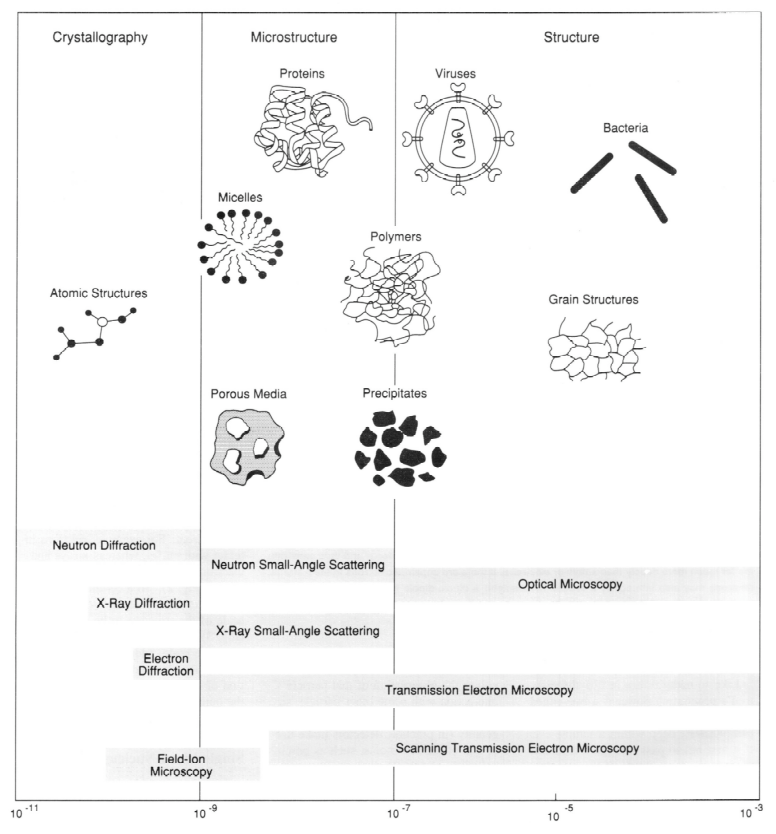
\includegraphics[width=\textwidth]{theory/length}
    \caption{A representation of how different techniques can be used to probe various length scales. Reprinted, with permission of Oxford University Press, from \cite{sivia_elementary_2011}.}
    \label{fig:lengths}
\end{figure}
%

Both X-ray and neutron scattering techniques are discussed and used in this work.
From an experimental viewpoint, there are significant differences between an X-ray scattering and a neutron scattering experiment.
However, there is little variation in terms of the data analysis, where the differences are limited to; the nature of the scattering lengths\footnote{See Section~\ref{convar}.} and the higher background that is present in the neutron scattering experiments.

\subsection{The scattering vector}
The scattering of some probing radiation,\footnote{Not just X-rays and neutrons, but any wave.} by some sample, can be represented as shown in Figure~\ref{fig:scat}.
Since only elastic scattering is being considered, there will be no change in the frequency of the radiation, $\omega_i = \omega_f$.
This means that only the wavevector, $\mathbf{k}$, can change, $\mathbf{k}_i\neq \mathbf{k}_f$.
The difference between the incident and final wavevectors is the scattering vector, $\mathbf{q}$, where,
%
\begin{equation}
    \mathbf{q} = \mathbf{k}_i - \mathbf{k}_f.
\end{equation}
%
%
\begin{marginfigure}
    \centering
    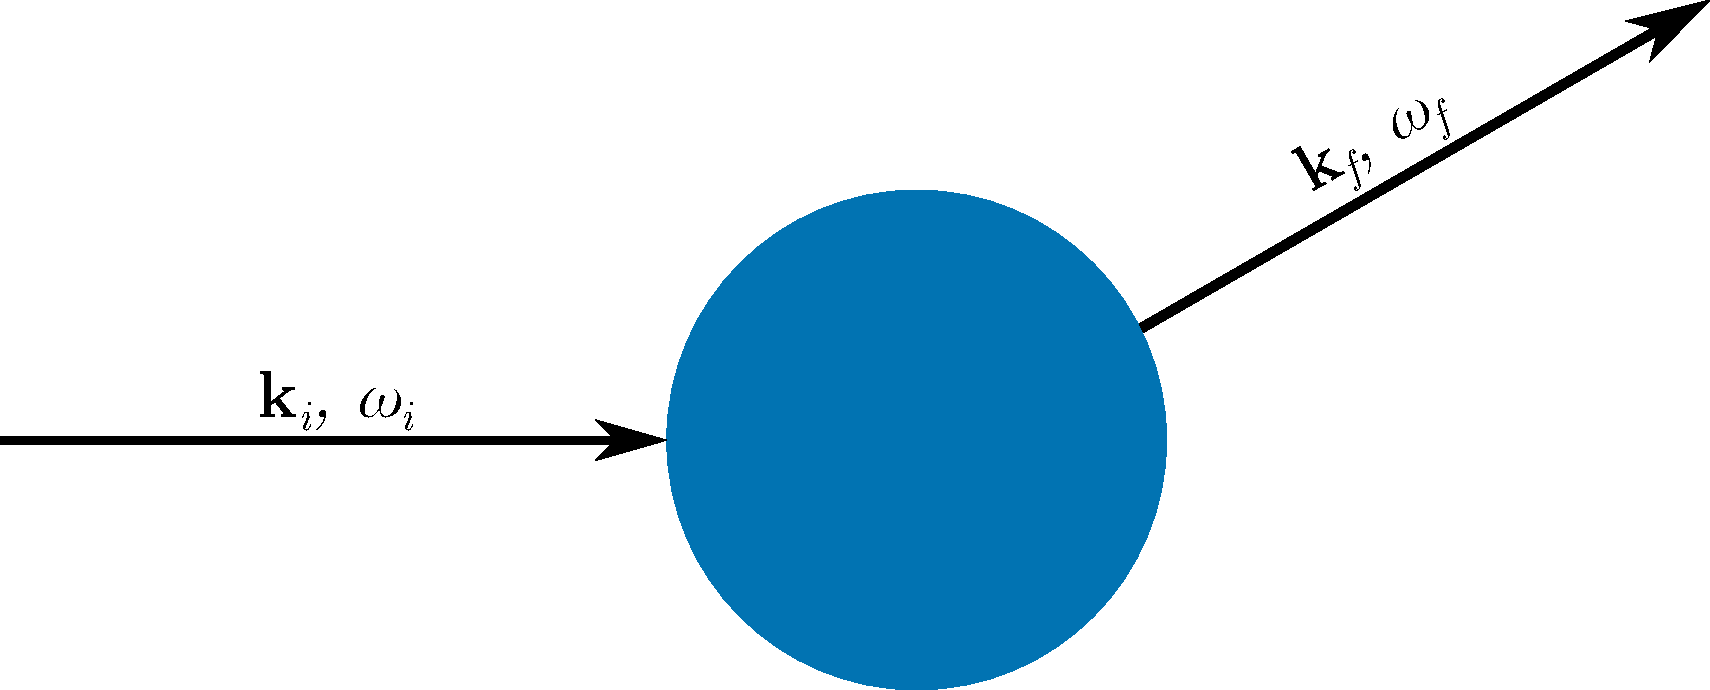
\includegraphics[width=\linewidth]{theory/scat}
    \caption{A schematic of the scattering of some probing radiation by a sample (blue circle). Adapted, with permission of Oxford University Press, from \cite{sivia_elementary_2011}.}
    \label{fig:scat}
\end{marginfigure}
%
The scattering vector strictly has units of \si{\per\meter}, however it is often more practical to use \si{\per\nano\meter} or \si{\per\angstrom}.\footnote{Throughout this work, units of \si{\per\angstrom} will be wherever possible.}
Since the frequency of the probing radiation does not change during an elastic scattering event, the wavelength, $\lambda$, will also not change, meaning that the moduli of the incident and final wavevectors are,
%
\begin{equation}
    |\mathbf{k}_i| = |\mathbf{k}_f| = \frac{2\pi}{\lambda}.
    \label{equ:wavevec}
\end{equation}
%
This also means that only the angle will change during the elastic scattering event.
The vector diagram in Figure~\ref{fig:scatvec} can be used to describe the geometry of an elastic scattering event.
From this, and Equation~\ref{equ:wavevec}, the value of $q$, where $q = |\mathbf{q}|$ can be shown as,
%
\begin{equation}
    q = \frac{4\pi\sin{\theta}}{\lambda}.
    \label{equ:theq}
\end{equation}
%
%
\begin{figure}[t]
    \centering
    \includegraphics[width=\textwidth]{theory/scatvec}
    \caption{A vector diagram describing an elastic scattering event, where $\mathbf{k}_i$ is the incident wavevector, $\mathbf{k}_f$ is the final wavevector, $2\theta$ is the scattering angle, and $\mathbf{q}$ is the scattering vector. Adapted, with permission of Oxford University Press, from \cite{sivia_elementary_2011}.}
    \label{fig:scatvec}
\end{figure}
%
However, this fails to fully capture the three dimensional nature of the scattering event.
Hence, it is necessary to describe the scattering with spherical coordinates, $2\theta$, and $\phi$, such that the incoming and outgoing radiation can be described as,
%
\begin{equation}
    \begin{aligned}
        \mathbf{k}_i & = \bigg(0, 0, \frac{2\pi}{\lambda}\bigg), \\
        \mathbf{k}_f & = \frac{2\pi}{\lambda}(\sin{2\theta}\cos{\phi}, \sin{2\theta}\sin{\phi}, \cos{2\theta}),
    \end{aligned}
\end{equation}
%
where, $|\mathbf{k}_f| = \sfrac{2\pi}{\lambda}$. This allows the scattering vector to be written,
%
\begin{equation}
    \mathbf{q} = \frac{4\pi\sin{\theta}}{\lambda}(-\cos{\theta}\cos{\phi}, -\cos{\theta}\sin{\phi},\sin{\theta}).
\end{equation}
%
For an isotropic scattering pattern, it is the magnitude of the scattering vector, $q$, that is measured.
In practical terms, the scattering vector allows for easy comparison of measurements made at different radiation wavelengths.

The basic quantity measured in a scattering experiment is the differential cross section, $\sfrac{\text{d}\sigma(q)}{\text{d}\Omega}$.
This is the fraction of particles of probing radiation that is scattered with a particular set of polar coordinates, $2\theta$ and $\phi$,
%
\begin{equation}
    \frac{\text{d}\sigma(q)}{\text{d}\Omega} = \frac{R_i(2\theta,\phi)}{NV\Phi\Delta \Omega},
    \label{equ:dsc}
\end{equation}
%
where, $R_i(2\theta,\phi)$ is the rate of arrival of the scattered particles at the position $2\theta$, $\phi$, $V$ is the illuminated volume of the sample, $\Phi$ is incident flux, $\Delta \Omega$ is some small solid angle, and $N$ is the number of scattering particles of interest, in the case of elastically scattered radiation, $N = N\%_{\text{el}}$, where $\%_{\text{el}}$ is the fraction of elastically scattered radiation.

\subsection{Scattering from a single fixed particle}
It is possible to describe a steady stream X-ray photons or neutrons of wavelength, $\lambda$, travelling through space as follows,
%
\begin{equation}
    \psi_i = \psi_o \exp{(\mathbf{i} kz)},
    \label{equ:wave}
\end{equation}
%
where, $z$ is the direction of travel, $k=\sfrac{2\pi}{\lambda}$, and the incident flux is the magnitude of the wave squared, $\Phi = |\psi_o|^2$.
This wave then interacts with a single fixed particle elastically, propagating the wave radially outwards, as shown in Figure~\ref{fig:singleatom}.
This propagation is centred on the atom, therefore the wavevector, $\mathbf{k_f}$ is parallel to the displacement vector, $\mathbf{r}$, and the following holds,
%
\begin{equation}
    \exp{(\mathbf{i}\mathbf{k}_f\cdot \mathbf{r})} = \exp{(\mathbf{i}kr)}.
\end{equation}
%
This final wave is no longer collimated and therefore diminishes with distance, $r$.
Hence the final scattered wave has the form,
%
\begin{equation}
    \psi_f = \psi_o b\frac{\exp{(\mathbf{i}kr)}}{r},
\end{equation}
%
where, $b$ is the scattering length discussed in Section~\ref{convar}.
%
\begin{marginfigure}
    \centering
    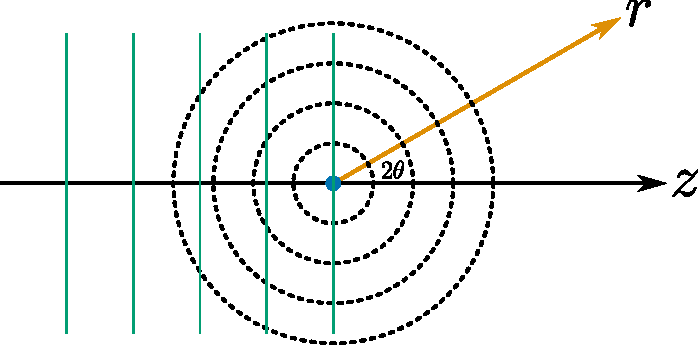
\includegraphics[width=\linewidth]{theory/singleatom}
    \caption{A schematic showing the propagation of the wave of probing radiation (green lines) radially outwards following the scattering event, where $r$ is the magnitude of the displacement vector. Adapted, with permission of Oxford University Press, from \cite{sivia_elementary_2011}.}
    \label{fig:singleatom}
\end{marginfigure}
%

\subsection{Scattering from multiple particles}
\label{sec:multiscat}

It is important to consider how the probing radiation would interact with a real system, consisting of many particles.
If the incident beam has the form of Equation~\ref{equ:wave}, with the wavevector $\mathbf{k}_i = (0, 0, k)$, each particle, $j$, will contribute the following to the total scattered wave, $\psi_f$, made up of the scattering from all, $N$, atoms,
%
\begin{equation}
    [\delta\psi_f]_j = \psi_o\exp{(\mathbf{ik}_i\cdot \mathbf{R}_j)}b_j\frac{\exp{\big\{\mathbf{ik}_f\cdot (\mathbf{r}-\mathbf{R}_j)\big\}}}{|\mathbf{r}-\mathbf{R}_j|},
\end{equation}
%
where, $\mathbf{R}_j$ is the position of particle $j$, $\mathbf{r}$ is some arbitrary position, and $\mathbf{k}_f$ is the wavevector of the scattered wave, described graphicall in Figure~\ref{fig:multiatom}.
This allows the total scattered wave to be defined as a summation of the contributions from the individual waves,
%
\begin{equation}
    \psi_f = \psi_o \exp{(\mathbf{ik}_f\cdot\mathbf{r})}\sum_{j=1}^{N}\bigg\{b_j \frac{\exp{(\mathbf{iq}\cdot \mathbf{R}_j)}}{|\mathbf{r}-\mathbf{R}_j|}\bigg\}.
    \label{equ:scatter}
\end{equation}
%
Equation~\ref{equ:scatter} holds true, within the Born approximation, where the scattered wave has no impact on the incident wave and each wave is scattered only once.
%
\begin{figure}[t]
    \forcerectofloat
    \centering
    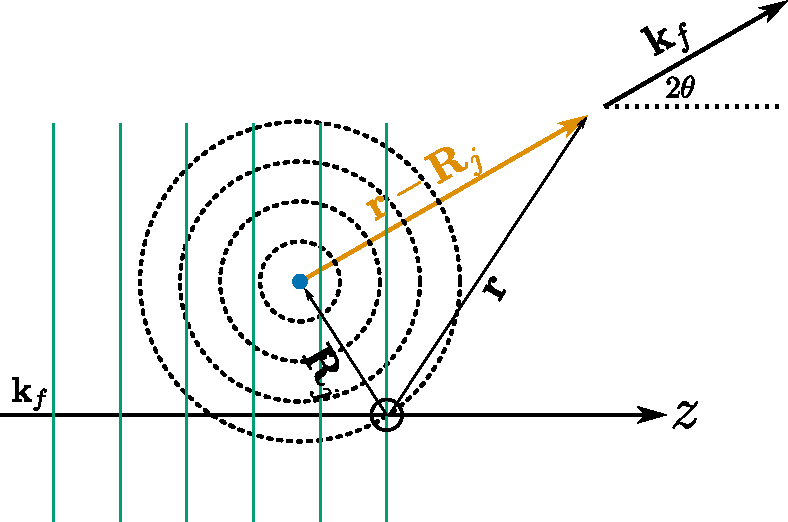
\includegraphics[width=\textwidth]{theory/multiatom}
    \caption{A schematic showing the interaction of radition scattered by two particles that are separated by the vector $\mathbf{R}_j$. Adapted, with permission of Oxford University Press, from \cite{sivia_elementary_2011}.}
    \label{fig:multiatom}
\end{figure}
%

The sample-detector distance is usually much larger than the typical particle size, allowing for the following approximation,
%
\begin{equation}
    |\mathbf{r} - \mathbf{R}_j| = |\mathbf{r}| = r.
\end{equation}
%
This is termed the Fraunhofer, or far-field limit, and allows Equation~\ref{equ:scatter} to be simplified,
%
\begin{equation}
    |\psi_f|^2 = \frac{\Phi}{r^2}\Bigg|\sum_{j=1}^{N}b_j\exp{(\mathbf{iq}\cdot\mathbf{R}_j)}\Bigg|^2.
\end{equation}
%
In the scattering experiment, radiation is deflected elastically into a detector with a small area, $\delta A$, at the polar coordinates, $2\theta$ and $\phi$, at a rate of $R_{\text{el}}$,
%
\begin{equation}
    R_{\text{el}}(2\theta,\phi) = |\psi_f|^2\delta A = \Phi\delta\Omega\Bigg|\sum_{j=1}^{N}b_j\exp{(\mathbf{iq}\cdot\mathbf{R}_j)}\Bigg|^2,
\end{equation}
%
where, $\delta\Omega = \sfrac{\delta A}{r^2}$.
Therefore, the differential cross section, defined in Equation~\ref{equ:dsc} can be related to the scattering from the sample as,
%
\begin{equation}
    \bigg(\frac{\text{d}\sigma(q)}{\text{d}\Omega}\bigg)_{\text{el}} = \frac{1}{V} \Bigg|\sum_{j=1}^{N}b_j\exp{(\mathbf{iq}\cdot\mathbf{R}_j)}\Bigg|^2.
    \label{equ:sca}
\end{equation}
%

\subsection{Scattering length density}
\label{sec:sld}
While it may be helpful to consider the scattering from multiple particles individually, where each particle has a scattering length, $b$.
In practice, due to low experimental resolution at small angles, it is more common to consider the SLD of the system,
%
\begin{equation}
    \text{SLD} = \frac{1}{V}\sum_{i=0}^{N} b_i,
\end{equation}
%
where $N$ is the total number of particles in the volume $V$.
A result of this equation is the ability to rewrite Equation~\ref{equ:sca} as,
%
\begin{equation}
    \bigg(\frac{\text{d}\sigma(q)}{\text{d}\Omega}\bigg)_{\text{el}} = \frac{1}{V} \Bigg|\iiint \limits_V \text{SLD}\exp{(\mathbf{iq}\cdot\mathbf{R})}\text{d}^3\mathbf{R}\Bigg|^2.
    \label{equ:sldsca}
\end{equation}
%
This equation shows that the scattering differential cross-section from some object is related to the SLD profile of that object by a Fourier transform.

\subsection{Model-dependent analysis}
\label{sec:moddep}
All types of scattering patterns can be analysed by two analysis methods; model independent and model-dependent.
Model-independent analysis is where there is no \emph{a priori} information used in the analysis, when there are no assumptions made about the underlaying structure of the sample. 
However, model-dependent analysis is when reasonable assumptions are made about the structure before the analysis is considered. 
The nature of this work means that it will focus on model-dependent analysis methods.\footnote{With the model usually being derived from some atomistic, or coarse-grained simulation.}
Model-dependent analysis has significant benefits over model-independent methods, such as improved resolution and more detailed information about the structure.
However, the necessity of the inclusion of \emph{a priori} information within model-dependent analysis may act to bias the result.
While this is undesirable, these assumptions can, and should, be educated based on the chemical information present.\sidecite[such as the propensity for twin-tailed phospholipid molecules to form monolayers at an air-water interface or small surfactants to form micelles in solution.]{mccluskey_model-dependent_2018}

The scattering from the model system is determined, using technique specific methods that are discussed in detail in later sections.
This is then compared with the experimental data using some figure of merit, the model is then varied to find the best possible model for the data provided.\footnote{This typically uses some optimisation algorithm to determine the best solution, the particular algorithms used in this work are discussed in Section~\ref{sec:optimisation}.}
In order to accurately reproduce the experimental measurement, it is necessary to include some instrumental resolution function, $res(q)$, in the modelling procedure.
This is instrument-specific, although it may be approximated by convolving the experimental dataset with some Gaussian smearing function, the modelled intensity can then be determined from,\autocite{nelson_towards_2013-1,nelson_towards_2014}
%
\begin{equation}
    I(q) = res(q) * \frac{\text{d}\sigma(q)}{\text{d}\Omega},
\end{equation}
%
where, $\sfrac{\text{d}\sigma(q)}{\text{d}\Omega}$ is the differential cross-section, a measure of the number of scattering particles hitting a given solid angle of the detector.

The aim of model-dependent analysis is to obtain a model for the system which agrees well with the experimentally measured scattering data while producing something that is chemically and physically relevant.

\subsection{Reflectometry}
\label{sec:refltheory}

Reflectometry involves the interaction of the probing radiation with some interface, from which the radiation is reflected.
The geometry of a reflectometry experiment is shown in Figure~\ref{fig:refgeo}, where the reflectometry instrument is in the horizontal configuration, ideal for the study of liquid interfaces.\footnote{Such at those investigated in Chapters~\ref{reflectometry1} and \ref{reflectometry2}.}
Reflectometry measurements give information about the structure perpendicular to the interface, the \emph{z}-dimension in Figure~\ref{fig:refgeo}, and therefore the analysis of reflectometry data is founded on the assumption that the layers will be completely homogenous in the plane of the interface, the \emph{xy}-plane in Figure~\ref{fig:refgeo}.
In reality, since the layers are usually not completely homogeneous, an average is obtained for the area in the radiation beam.
%
\begin{figure}[t]
    \forcerectofloat
    \centering
    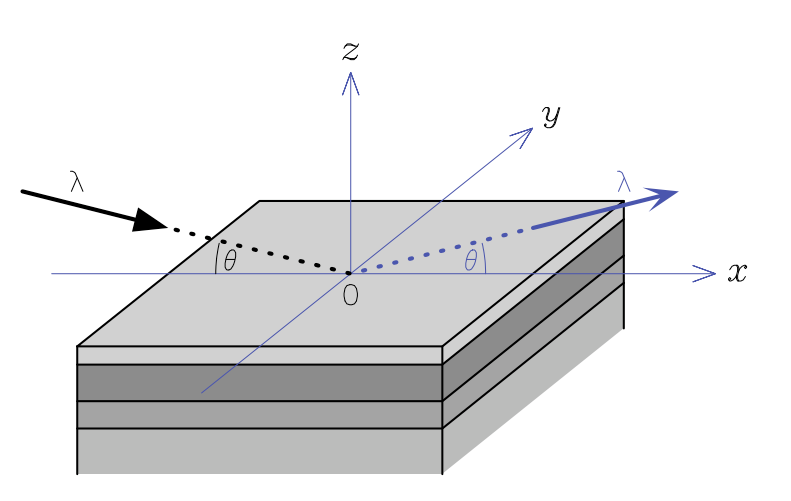
\includegraphics[width=0.8\textwidth]{theory/reflectgeo}
    \caption{A schematic showing the geometry of a typical specular reflectometry experiment from a layered sample. Reprinted, with permission of Oxford University Press, from \cite{sivia_elementary_2011}.}
    \label{fig:refgeo}
\end{figure}
%

A reflectometry instrument operates by measuring the intensity of specular reflected radiation at a series of different angles, $\theta$, or wavelengths, $\lambda$.
The reflected intensity is described in terms of the $q$-vector\footnote{Using Equation~\ref{equ:theq}}, and is defined as follows,
%
\begin{equation}
    R(q) = \frac{\text{specular reflected radiation intensity at }q}{\text{incident radiation intensity}}.
    \label{equ:refl}
\end{equation}
%
It is clear from Equation~\ref{equ:refl} that the value of the measured reflectometry cannot be greater than one, as this would mean that more particles of probing radiation were being reflected than were incident.

There are two model-dependent analysis techniques that can be applied to the understanding of a reflectometry dataset.
The first is the kinematic approach, which can be described with Equation~\ref{equ:sca}, from the assumption that $q_x = 0$ and $q_y = 0$, as only the specular scattering is being measured.
This approach models the reflectometry as a function of the SLD profile in the \emph{z}-dimension, $\text{SLD}(z)$,
%
\begin{equation}
    R(q) \approx \frac{16\pi^2}{q^4}\bigg|\int_{-\infty}^{+\infty}\frac{\text{d}\text{SLD}(z)}{\text{d}z}\exp{(-\mathbf{i}zq_z)}\text{d}z\bigg|^2,
    \label{kine}
\end{equation}
%
where, $\sfrac{\text{d}\text{SLD}(z)}{\text{d}z}$ is the first derivative of the SLD profile.
However, this method has a significant problem, which can be demonstrated by applying Equation~\ref{kine} to the SLD profile of a bare silicon substrate, which can be modelled as a Heaviside function, as shown in Figure~\ref{fig:kine}(a),
%
\begin{equation}
    \text{SLD}(z) =
  \begin{cases}
    0, & \text{where}\ z < 0 \\
    \text{SLD}_{\text{Si}}, & \text{otherwise}
  \end{cases}
\end{equation}
%
where, $\text{SLD}_{\text{Si}}$ is the SLD of pure silicon.\footnote{This is \SI{2.1e-6}{\angstrom^{-2}} for neutrons.}
The derivative of a stepwise Heaviside function is a scaled $\delta$-function, as shown in Figure~\ref{fig:kine}(b),
%
\begin{equation}
    \text{SLD}'(z) = \text{SLD}_{\text{Si}}\delta(z).
\end{equation}
%
Then, as in Equation~\ref{kine}, the Fourier transform of this $\delta$-function is taken,
%
\begin{equation}
    \text{SLD}_{\text{Si}}\int_{-\infty}^{+\infty}\delta(z)\exp{(-\mathbf{i}zq_z)}\text{d}z = \text{SLD}_{\text{Si}}\exp(0) = \text{SLD}_{\text{Si}}.
    \label{equ:rhosi}
\end{equation}
%
This means that, using Equations~\ref{equ:rhosi} and \ref{kine}, the reflectometry profile could be calculated from the following relationship,
%
\begin{equation}
    R(q)\approx \frac{16\pi^2\text{SLD}_{\text{Si}}^2}{q_z^4}.
\end{equation}
%
The curve from this relationship is shown in Figure~\ref{fig:kine}, where it is clear that the agreement with an experimental profile would be poor as $q \rightarrow 0$.
It can be seen that for low values of $q$ the calculated reflectometry is greater than 1, which violates the physical constraint imposed with Equation~\ref{equ:refl}.
This break down of the kinematic approach is due to the assumption present in this approach that the Born approximation\footnote{Mentioned previously in Section~\ref{sec:multiscat}.} will hold.
However, in the reflectometry scattering geometry, this is no longer true rendering the kinematic approach invalid.
%
\begin{figure}[t]
    \centering
    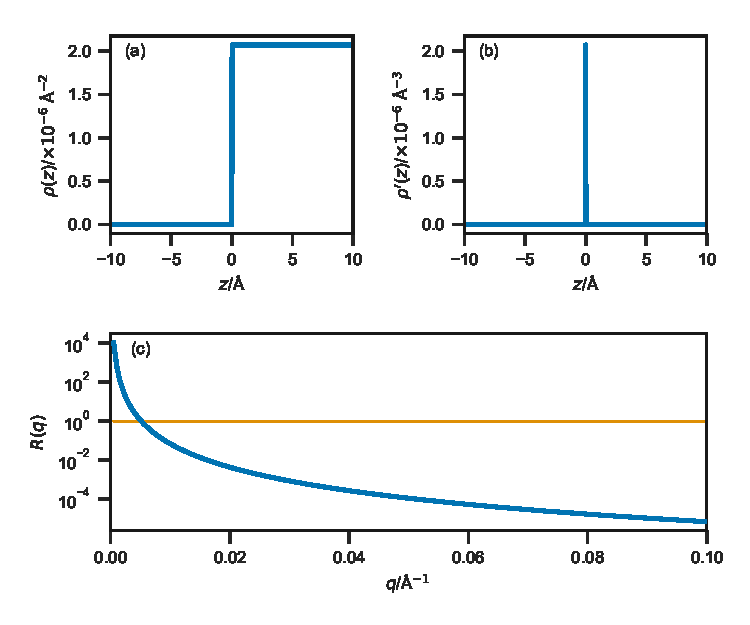
\includegraphics[width=\textwidth]{theory/kine}
    \caption{A graphical representation of the kinematic approach; (a) the Heaviside function describing the SLD profile of a bare silicon substrate, (b) the $\delta$-function arising from the first derivative of the function in (a), and (c) the reflectometry profile resulting from the kinemtic approach, where the orange line at $R=1$ identifies the break down between experimental and theory in the kinematic approach. Adapted, with permission of Oxford University Press, from \cite{sivia_elementary_2011}.}
    \label{fig:kine}
\end{figure}
%

This breakdown of the kinematic approach has led to the application of the Abel\`{e}s, or Parratt, model for the reflection of light at a given number of stratified interfaces.\sidecite[also known as dynamical theory]{abeles_sur_1948,parratt_surface_1954}
This method involves considering the system as a layered structure at the interfaces of which, the probing radiation can either be reflected or refracted, by some refractive index, $n_i$.
Figure~\ref{fig:reflrefr} shows this process for a system of two layers, where the layer \num{0} is the air or vacuum above the sample, it is clear to see how the two waves labelled $r$ could interfere constructively or destructively depending on the thickness of layer \num{1}, $d$.
This means that for a single interface,\footnote{Such as that between layers \num{0} and \num{1} in Figure~\ref{fig:reflrefr}.} the reflectometry can be described by the Fresnel equation,
%
\begin{equation}
    R(q) = \bigg| \frac{n_0\sin{\theta_0} - n_1\sin{\theta_1}}{n_0\sin{\theta_0} + n_1\sin{\theta_1}} \bigg|^2.
\end{equation}
%
Additionally at the point of total reflection, where $\theta_0 = \theta_{\text{c}}$, the critical angle, there will be no transmitted wave so,
%
\begin{equation}
    n_1\sin{\theta_1} = 0,
\end{equation}
%
and therefore the reflected radiation will never be greater than 1, while the critical angle can be defined as,
%
\begin{equation}
    \cos^2{\theta_{\text{c}}} = \frac{n_1^2}{n_0^2}.
\end{equation}
%
This is the angle below which a reflectometry profile will be measured.
%
\begin{figure}[t]
    \centering
    \includegraphics[width=\textwidth]{theory/reflrefr}
    \caption{A schematic diagram showing the reflected ($r$) and transmitted ($t$) waves when an incident ($i$) wave enters an interface of thickness $d$, where the refractive indices of each layer are $n_0$, $n_1$, and $n_2$. Adapted, with permission of Elsevier, from \cite{foglia_studies_2015}.}
    \label{fig:reflrefr}
\end{figure}
%

%
\begin{figure}[t]
    \forceversofloat
    \centering
    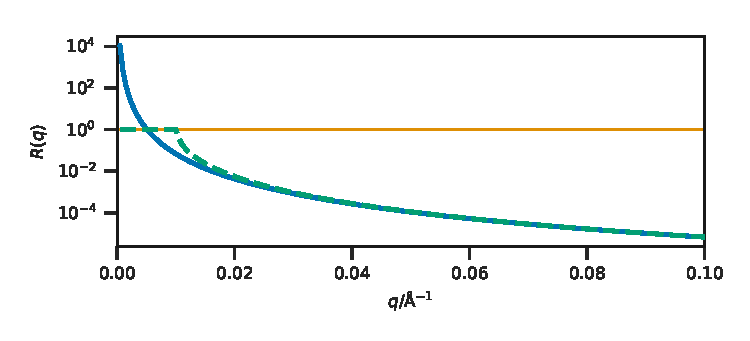
\includegraphics[width=\textwidth]{theory/dyna}
    \caption{A comparison of the kinematic approach (blue solid line), and the dynamical approach (green dashed line), to determine the reflected intensity from the material with the SLD profile given in Figure~\protect\ref{fig:kine}(a). It is clear that at low $q$, there is a noticable deviation between the two.}
    \label{fig:dyna}
\end{figure}
%
The above method can then be generalised to a structure of an arbitrary number of layers, as shown in Code Block~\ref{cb:refl}.\footnote{The purpose of the Code Blocks throughout this work is to ensure transparency and reproducibility, these are written as Python functions.}
For each value of $q$ for which the reflectometry is to be calculated, the system is considered in terms of $n_{\text{max}}$ layers.
The incident radiation beam will be refracted by each of the layers, giving wavevectors values for each layer, $k_n$,
%
\begin{equation}
    \label{equ:knsld}
    k_n = \sqrt{k_0^2 + 4\pi (\text{SLD}_n - \text{SLD}_0)},
\end{equation}
%
where, $k_0=\sfrac{q}{2}$.
The Fresnel equation coefficient between layers $n$ and $n+1$, $r_{n,n+1}$ can then be found along with the phase factor, $\beta_n$, as the Born approximation holds for SAS, which is dependent on the thickness of the layer, $d_n$,
%
\begin{equation}
    r_{n,n+1} = \frac{k_n - k_{n+1}}{k_n + k_{n+1}},
    \label{equ:fres}
\end{equation}
%
%
\begin{equation}
    \label{equ:nowthick}
    \beta_n = k_n d_n.
\end{equation}
%
The means that a matrix can be evaluated for each layer, $M_n$,
%
\begin{equation}
    M_n =
    \begin{bmatrix}
        \exp{\beta_n} & r_{n,n+1}\exp{-\beta_n} \\ r_{n,n+1}\exp{\beta_n} & \exp{-\beta_n}
    \end{bmatrix}
\end{equation}
%
The resultant matrix, $B$, is then found as a product of the matrix from each layer,
%
\begin{equation}
    B = \prod_{n=0}^{n_{\text{max}}} M_n,
\end{equation}
%
and from this the reflected intensity at the given value of $q$ can be found,
%
\begin{equation}
    R(q_z) = \frac{B_{1,2}}{B_{1,1}}.
\end{equation}
%
This algorithm models the layers as perfectly flat layers, which will not be strictly true.\footnote{Particularly for soft matter systems.}
This resulted in the correction term being added to Equation~\ref{equ:fres} to account for the roughness of the layers.
This adapts Equation~\ref{equ:fres} to the form,
%
\begin{equation}
    r_{n,n+1} = \frac{k_n - k_{n+1}}{k_n + k_{n+1}}\exp{(-2k_nk_{n+1}\sigma^2_{n,n+1})},
\end{equation}
%
where, $\sigma_{n,n+1}$ is the interfacial roughness between layers $n$ and $n+1$.\sidecite<-2\baselineskip>{nevot_caracterisation_1980}
This has the effect of Gaussian broadening the layers into each other, as a result.
This method\sidenote[][-1.5\baselineskip]{That is given programmatically in Code Block~\protect\ref{cb:refl}.} is currently implemented in a variety of reflectometry modelling software packages, such as \texttt{refnx}, MOTOFIT, RasCAL, and Aurore \sidecite<-2\baselineskip>{nelson_refnx_2019,nelson_co-refinement_2006,hughes_rascal_nodate,gerelli_aurore_2016-1,gerelli_aurore_20162}.
Applying this method to the SLD profile shown in Figure~\ref{fig:kine} gives the reflectometry profile shown with the dashed green line in Figure~\ref{fig:dyna}.
%
\begin{listing}[t]
    \forcerectofloat
    \centering
    \caption{An example Python code block for the Abel\`{e}s method for the calculation of reflectometry, adapted from \cite{nelson_refnx_2019}. The input variables are \texttt{q\_values} which are the $q$-vectors at which the reflected intensity should be calculated, \texttt{sld} which is the array of scattering length densities for the layers, and \texttt{d} which is the array of thicknesses for the layers. This will return an array of floats that is the same size as the \texttt{q\_values} and contains the reflected intensities.}
    \lstinputlisting[nolol]{reports/code_blocks/reflectometry.py}
    \label{cb:refl}
\end{listing}
%

\subsection{Small angle scattering}
\label{sec:sasanal}

Equation~\ref{equ:sldsca} identified that the scattering differential cross-section for some object was related to the SLD by a Fourier transform, which is shown graphically in Figure~\ref{fig:scales}.
This figure shows that there is a reciprocal relationship between the size of the object and the scattered intensity, decaying significantly up to values of $2\pi/d_x$, where $d_x$ is the size of the object.
This means that in order to probe large-scale structural features that are of interest in the study of soft materials, it is necessary to consider small values of $q$.
When considering the nature of $q$ in Equation~\ref{equ:theq}, it is clear that such experiments would benefit from small values of $\theta$ and large values of $\lambda$.
Hence, the use of scattering at small angles.
%
\begin{marginfigure}
    \centering
    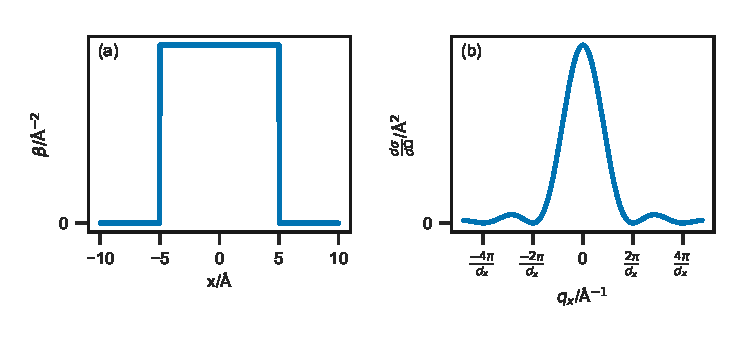
\includegraphics[width=\linewidth]{theory/scales}
    \caption{The effect of a Fourier transform (a) the SLD profile for some object with a width of \SI{10}{\angstrom}, (b) the Fourier transform of this object showing the minima in the differential cross section at values of $\sfrac{2n\pi}{10}$, where $n$ is some integer.}
    \label{fig:scales}
\end{marginfigure}
%

A SAS experiment generally involves some sample being placed in the path of the probing radiation; the scattering pattern that results from this transmission is measured at some distance, as is shown in Figure~\ref{fig:sasgeo} for the D22 SANS instrument of the ILL.
SAS instruments are usually very large, due to the large post sample flight path that is necessary to reach the small angles being measured.\footnote{A longer flight path allows more space for angular divergence.}
Transmission SAS can provide information about the size, shape and orientation of the sample's components.\autocite{willis_experimental_2009}
The range of $q$ that is typically covered by a SAS instrument is usually around \SIrange{2e-3}{0.5}{\per\angstrom}, which corresponds to \SIrange{10}{3000}{\angstrom} in real-space.
The neutron or X-ray detector of a SAS instrument is often two-dimensional, meaning that for an isotropic scattering profile, the detector image is radially averaged to give an $I(q)$ scattering profile.
It is possible to increase the $q$-range of a SAS instrument through the introduction of wide-$q$ detector banks close to the sample or small-$q$ detector banks further away.
This allows the SANS2D instrument, at the ISIS Neutron and Muon Source, to have a total range from \SIrange{2e-3}{2}{\per\angstrom}.\autocite{noauthor_isis_nodate}
Furthermore, the SANS2D instrument may leverage the ToF method discussed in Section \ref{sec:neutrons} to allow for a much shorter post sample flight path than is present at D22.
%
\begin{figure}[t]
    \centering
    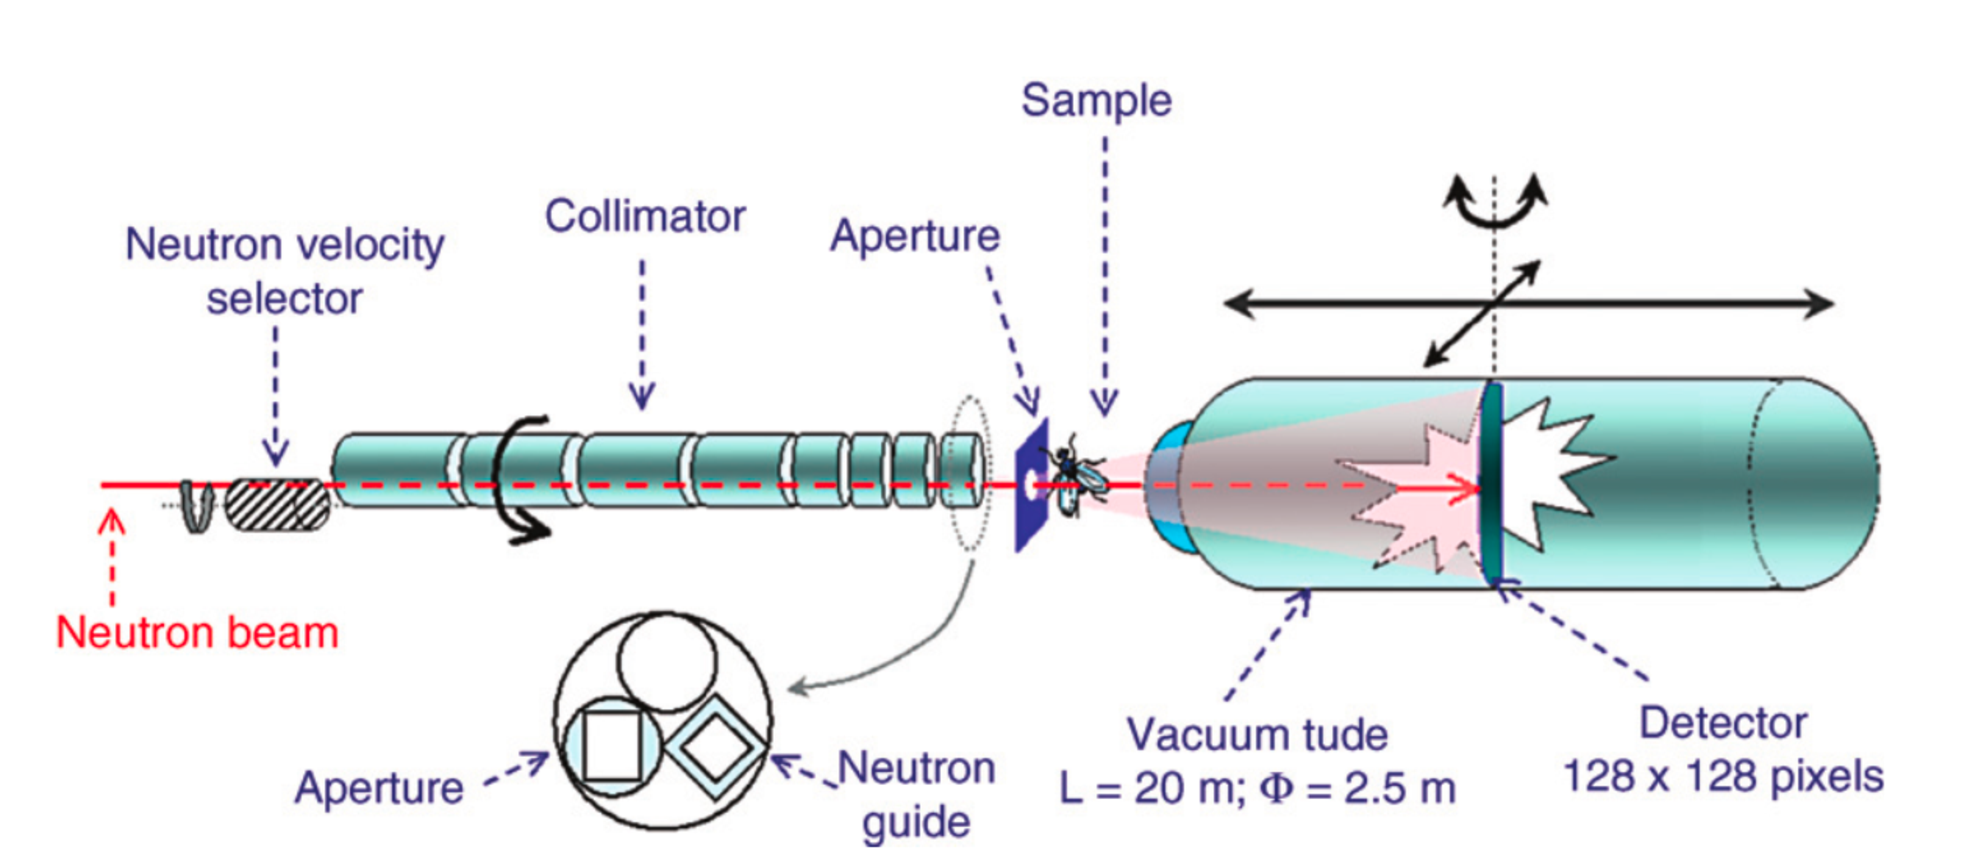
\includegraphics[width=\textwidth]{theory/d22}
    \caption{A schematic of the D22 instrument of the ILL. Reprinted with permission of Springer Nature Customer Service Centre GmbH: Springer Nature from \cite{grillo_small-angle_2008}.}
    \label{fig:sasgeo}
\end{figure}
%

A radially averaged SAS pattern can be considered as consisting of two sections that arise from the form and structure factors for the scattering species.
The form factor gives information about the average shape of the scattering particle, while the structure factor is a measure of the interaction present between the objects.
It is often possible to control the presence of the structure factor by changing the concentration of the sample, eventually, the concentration will be so low that all interparticle interaction is screened by the solvent.\autocite{edler_combining_2015}
This method is frequently applied in biological SAXS applications, where the interactions between the protein molecules are of less interest than the overall structure of the complex.
However, with micelles, it is not always possible to remove the structure factor, as the critical micelle concentration may be higher than the minimum concentration at which the structure factor is present.
It is possible to deconvolute the structure and form factors for a micellar solution by studying different concentrations, assuming that the form of the micelle is concentration independent, over the measured concentration range.

The rigorous, model-independent method for the analysis of SAS involves taking the inverse Fourier transform of the scattering profile, to give an auto-correlation function of the average particle in the system, which following a deconvolution procedure will resolve the radially averaged SLD profile.
However, this is often cumbersome and has a low information density, when compared to model-dependent techniques.
Additionally, if the experimental data lacks information at wide enough $q$ to cover all features of the sample, artefacts may be present in the inverse Fourier transform of the scattering.

There are two common and straight-forward analysis procedures that can be used to give an understanding of the scattering species structure.
The first is the Guinier approximation, which is used in the determination of the radius of gyration, $R_g$, of the scattering species at ``infinite dilution''.
This scattering law is only valid at very small values of $q$, where $q < R_g^{-1}$,\autocite{sivia_elementary_2011}
%
\begin{equation}
    \ln[I(q)] = \ln[I(0)] - \Bigg(\frac{R_g^2}{3}\Bigg)q^2.
\end{equation}
%
This relationship allows the radius of gyration to be found by plotting the scattering profile transformed into $\ln[I(q)]$ vs. $q^2$, and evaluating the gradient at low $q$.
The Guinier plot for the scattering from a sphere with a radius of \SI{20}{\angstrom} is shown in Figure~\ref{fig:rg}, where the radius of gyration correlates with the radius of the sphere, $R_s$, as follows,
%
\begin{equation}
    R_g = \sqrt{\frac{3}{5}}R_s.
\end{equation}
%
The Guinier analysis is very common in the study of proteins by SAS, as it allows for the determination of the protein size in the native, solution phase.\autocite{skou_synchrotron-based_2014}
Another common analysis of SAS data comes in the form of Porod's law, which states that for large values of $q$, the scattering intensity becomes proportional to $Sq^{-4}$, where $S$ is the surface area of the sample.
This means that by plotting $I(q)q^4$ vs. $q$ and extrapolating to $q \rightarrow \infty$, it is possible to determine the external surface area of the system.\autocite{willis_experimental_2009}
Using the surface area, it is then possible to qualitatively determine the ``roughness'' of the system based on the relation of the surface area to the particle size.
%
\begin{figure}[t]
    \centering
    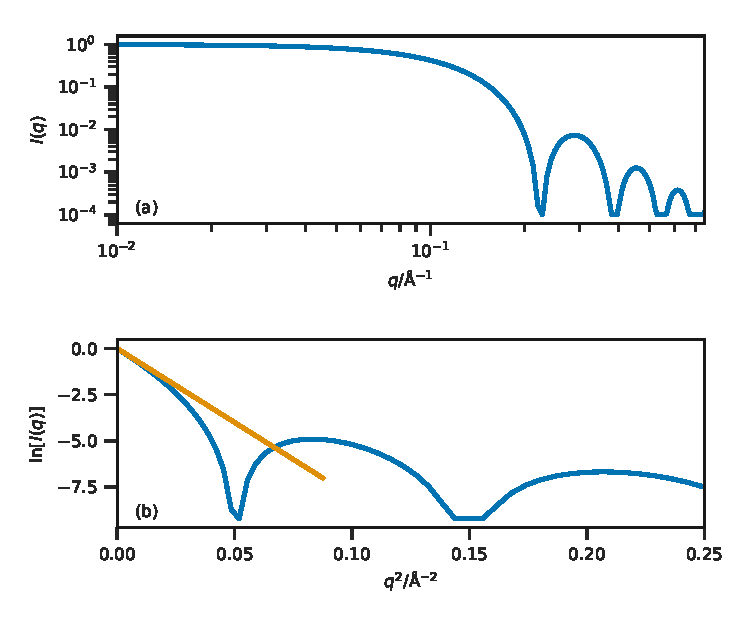
\includegraphics[width=\textwidth]{theory/rg}
    \caption{The Guinier plot, (a) the ideal scattering profile from a sphere of radius \SI{20}{\angstrom}, (b) the associated Guinier plot, with a straight line (orange) at low-$q$ showing the radius of gyration to be \SI{\sim15.5}{\angstrom}.}
    \label{fig:rg}
\end{figure}
%

In the calculation of a SAS pattern, both the structure and form factors will contribute.
Therefore, when the pattern is modelled, the differential cross-section, which is measured experimentally, has the following form.\footnote{When the system is centrosymmetric.}
%
\begin{equation}
    \frac{\text{d}\sigma(q)}{\text{d}\Omega} = N_\rho\Delta\text{SLD}^2V_p^2 P(q)S(q),
\end{equation}
%
where $N_\rho$ is the number density of the particles, $\Delta\text{SLD}$ is the difference in scattering length density between the particles and the solvent, $V_p$ is the particle volume, $P(q)$ is the particle form factor, and $S(q)$ is the structure factor.\autocite{pedersen_monte_2002}
Therefore, it is necessary to understand the form and structure factors individually.

The most common method for the modelling of the form factor is by using very coarse shapes; such as spheres, cylinders, or ellipses.
This involves the evaluation of analytical or quasi-analytical solutions for the scattering, which have been derived for many common shapes.
The solution for a sphere was solved in the early 19th century by Lord Rayleigh.\autocite{pedersen_monte_2002}
%
\begin{equation}
    P(q) = \Bigg\{\frac{3\big\{\sin(qR_s) - qR\cos(qR_s)\big\}}{(qR_s)^3}\Bigg\}^2,
    \label{equ:sphere}
\end{equation}
%
where $R_s$ is the radius of the sphere.
A comparison between a possible experimental scattering pattern and the scattering generated from Equation~\ref{equ:sphere} is shown in Figure~\ref{fig:sphere}.
Analytical form factors exist for a wide variety of shapes; these can be found in software such as SASView and SASFit.\autocite{noauthor_sasview_nodate, noauthor_sasfit_nodate}
%
\begin{figure}[t]
    \centering
    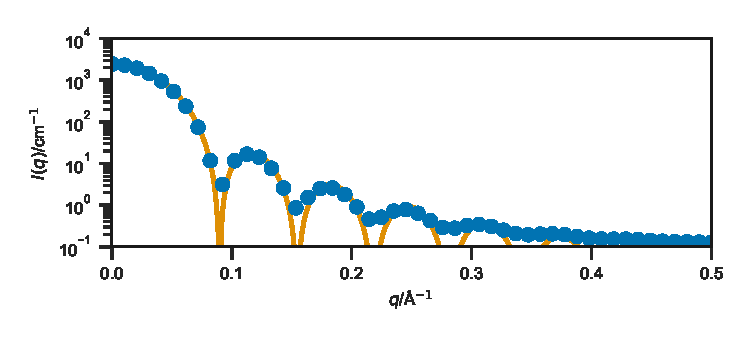
\includegraphics[width=\textwidth]{theory/sphere}
    \caption{The SANS profile of a micelle of \ce{C_{16}TAB} with radius $\SI{50(3)}{\angstrom}$ (circles, generated using SASView \cite{noauthor_sasview_nodate}, with instrumental smearing) compared with a curve of Equation~\protect\ref{equ:sphere}, where $R = \SI{50}{\angstrom}$ (solid line).}
    \label{fig:sphere}
\end{figure}
%

The structure factor accounts for the scattering interference that arises from the interaction of different particles.
This is modelled using expressions which depend on the nature of the scattering particles; hard-sphere, sticky hard-spheres, screened Coulomb, etc.
Structure factor expressions are generated as solutions to the Ornstein-Zernike Equation.\autocite{klein_interacting_2002}
The most relevant structure factor in terms of micelle modelling is probably the Hayter-Penfold Mean Spherical Approximation, \autocite{hayter_analytic_1981} this is where the micelles are modelled as like-charged, soft spheres and is valid for dilute solutions.
Again, a whole range of these structure factor functions are built into the SASView package.\autocite{noauthor_sasview_nodate}

In order to evaluate the scattering profile from an atomic structure,\footnote{Or any coordinate system, such as a coarse-grained simulation.} it is possible to use the Debye equation.\autocite{debye_zerstreuung_1915}
This is an analytical relationship for the determination of the scattering profile based on the atomic positions, $\mathbf{r}_i$,
%
\begin{equation}
    I(q) = \sum_{i}^{N}\sum_{j}^{N} b_ib_j\frac{\sin{(q|\mathbf{r}_i-\mathbf{r}_j|)}}{q|\mathbf{r}_i-\mathbf{r}_j|},
\end{equation}
%
where, $N$ is the number of particles, $q$ is the scattering vector, and $b_i$ and $b_j$ are the scattering lengths of particles $i$ and $j$ respectively.\footnote{In the case of a coarse-grained particle, this can be obtained from summing the scattering lengths of the constituent atoms.}
The Debye equation is powerful, however, it is not intrinsically parallelisable and scales as $\mathcal{O}(N^2)$.
In order to improve the efficiency of the calculation of the scattering profile, a variety of methods have been developed that offer a sufficiently accurate approximation.\autocite{svergun_solution_1994,watson_rapid_2013}
The Golden Vector method, developed by Watson and Curtis,\autocite{watson_rapid_2013} scales as $\mathcal{O}(Nn)$, where $n$ is the number of scattering vectors used in the calculation.
In this method, the scattering amplitude is calculated numerically for a single $\mathbf{q}$-vector,
%
\begin{equation}
    I(\mathbf{q}) = \Bigg[\sum_{i}^{N}b_i\cos{(\mathbf{q}\cdot\mathbf{r}_i)}\Bigg]^2 + \Bigg[\sum_{i}^{N}b_i\sin{(\mathbf{q}\cdot\mathbf{r}_i)}\Bigg]^2.
\end{equation}
%
This is carried out for $n$ scattering vectors that are selected in an orientationally averaged fashion from a quasi-uniform lattice on a sphere.
This was first developed such that $n$ is a number from the Fibonacci sequence,\autocite{svergun_solution_1994} however for the Golden Vector method, $n$ may be any positive integer.
This leads to the scattering vectors being calculated as,
%
\begin{equation}
    \begin{aligned}
        q_x^{(k)} & = q\cos\Bigg[\sin^{-1}\bigg(\frac{2k}{n}\bigg)\Bigg]\cos\bigg(\frac{2\pi k}{\Phi}\bigg), \\
        q_y^{(k)} & = q\cos\Bigg[\sin^{-1}\bigg(\frac{2k}{n}\bigg)\Bigg]\sin\bigg(\frac{2\pi k}{\Phi}\bigg), \\
        q_z^{(k)} & = \frac{2 k q}{n},
    \end{aligned}
\end{equation}
%
where, $k$ runs from $-(n-1)/2,\ldots,0,\ldots,(n-1)/2$ and $\Phi$ is the golden ratio,
%
\begin{equation}
    \Phi = \frac{1+\sqrt{5}}{2}.
\end{equation}
%
The approximate orientationally averaged scattering is then found as an average of the scattering from each of ther individual $q$-vectors,
%
\begin{equation}
    I(q) = \frac{1}{n}\Bigg\{\sum_{k=(1-n)/2}^{(n-1)/2} I[\mathbf{q}^{(k)}]\Bigg\}.
\end{equation}
%
The accuracy of this calculation increases with $n$, however agreement, comparible to the Debye equation, between experiment and simulation has been shown for $n < 100$ even for highly anisotropic systems.\autocite{watson_rapid_2013}
